\chapter{Single-Neuron and Population Models}
\label{ch:single-neuron-population-models}

\textit{A spiking neuron is not a rate unit. This chapter shows how a voltage
model emits discrete spikes, how stochasticity turns threshold crossing into a
probabilistic input-output relation, and how finite populations of LIF/GIF
neurons become mesoscopic activity equations only after averaging, filtering,
and adding the correct finite-size fluctuations.}

% ============================================================
\section{Why Start with a Single Neuron?}
\label{sec:why-single-neuron}
% ============================================================

The previous chapters introduced two languages we now need simultaneously:
trajectories in a state space and random point events in time. A cortical circuit
uses both. The membrane voltage of a neuron evolves continuously, but the
neuron communicates mostly through spikes, which are discrete events. A rate
description is therefore not a microscopic law. It is a summary of spike
statistics after some combination of time averaging, population averaging, and
conditioning on an input.

This distinction matters for clustered networks. Later we will describe the
activity of a cluster by a time-dependent population rate. That rate is useful
because a cluster contains many neurons. It is not useful because an individual
neuron secretly follows a deterministic rate equation. The purpose of this
chapter is to make that passage precise enough that the later mean-field and
mesoscopic approximations have a clear microscopic meaning.

The derivation ladder used here is the one needed for clustered-network work:
voltage and history variables define an escape rate; escape rates define an
age-density or renewal equation for population activity; finite population size
adds an activity noise term with amplitude \(1/\sqrt{N}\); filtering then maps
raw spikes into the cluster rates used in simulations.

% ============================================================
\section{The Leaky Integrate-and-Fire Model}
\label{sec:lif}
% ============================================================

The leaky integrate-and-fire (LIF) model keeps the part of neuronal biophysics
that is essential for network theory: currents charge a membrane capacitance,
leak pulls voltage back toward rest, and a spike is emitted when the voltage
crosses a threshold. Between spikes,
%
\begin{keyequation}[Leaky Integrate-and-Fire Voltage]
\begin{equation}
  \tau_m \frac{dV_i}{dt}
  =
  -\bigl(V_i(t)-E_L\bigr)
  + R_m I_i(t),
  \qquad
  V_i(t^-)=V_\theta \Rightarrow
  \begin{cases}
    \text{emit a spike at }t,\\
    V_i(t^+)=V_r.
  \end{cases}
  \label{eq:ch03-lif-voltage}
\end{equation}
\tcblower
$V_i$: membrane potential of neuron $i$; $\tau_m$: membrane time constant;
$E_L$: leak reversal or resting voltage; $R_m$: membrane resistance;
$I_i(t)$: synaptic plus external input current; $V_\theta$: threshold;
$V_r$: reset voltage.
\end{keyequation}

\noindent The equation is linear until threshold. The nonlinearity is the reset
rule: a continuous voltage trajectory is converted into a point event and then
returned to a lower voltage. Thus the LIF model separates two jobs. The
differential equation describes subthreshold integration; the threshold/reset
condition defines the spike train.

\begin{figure}[t]
\centering
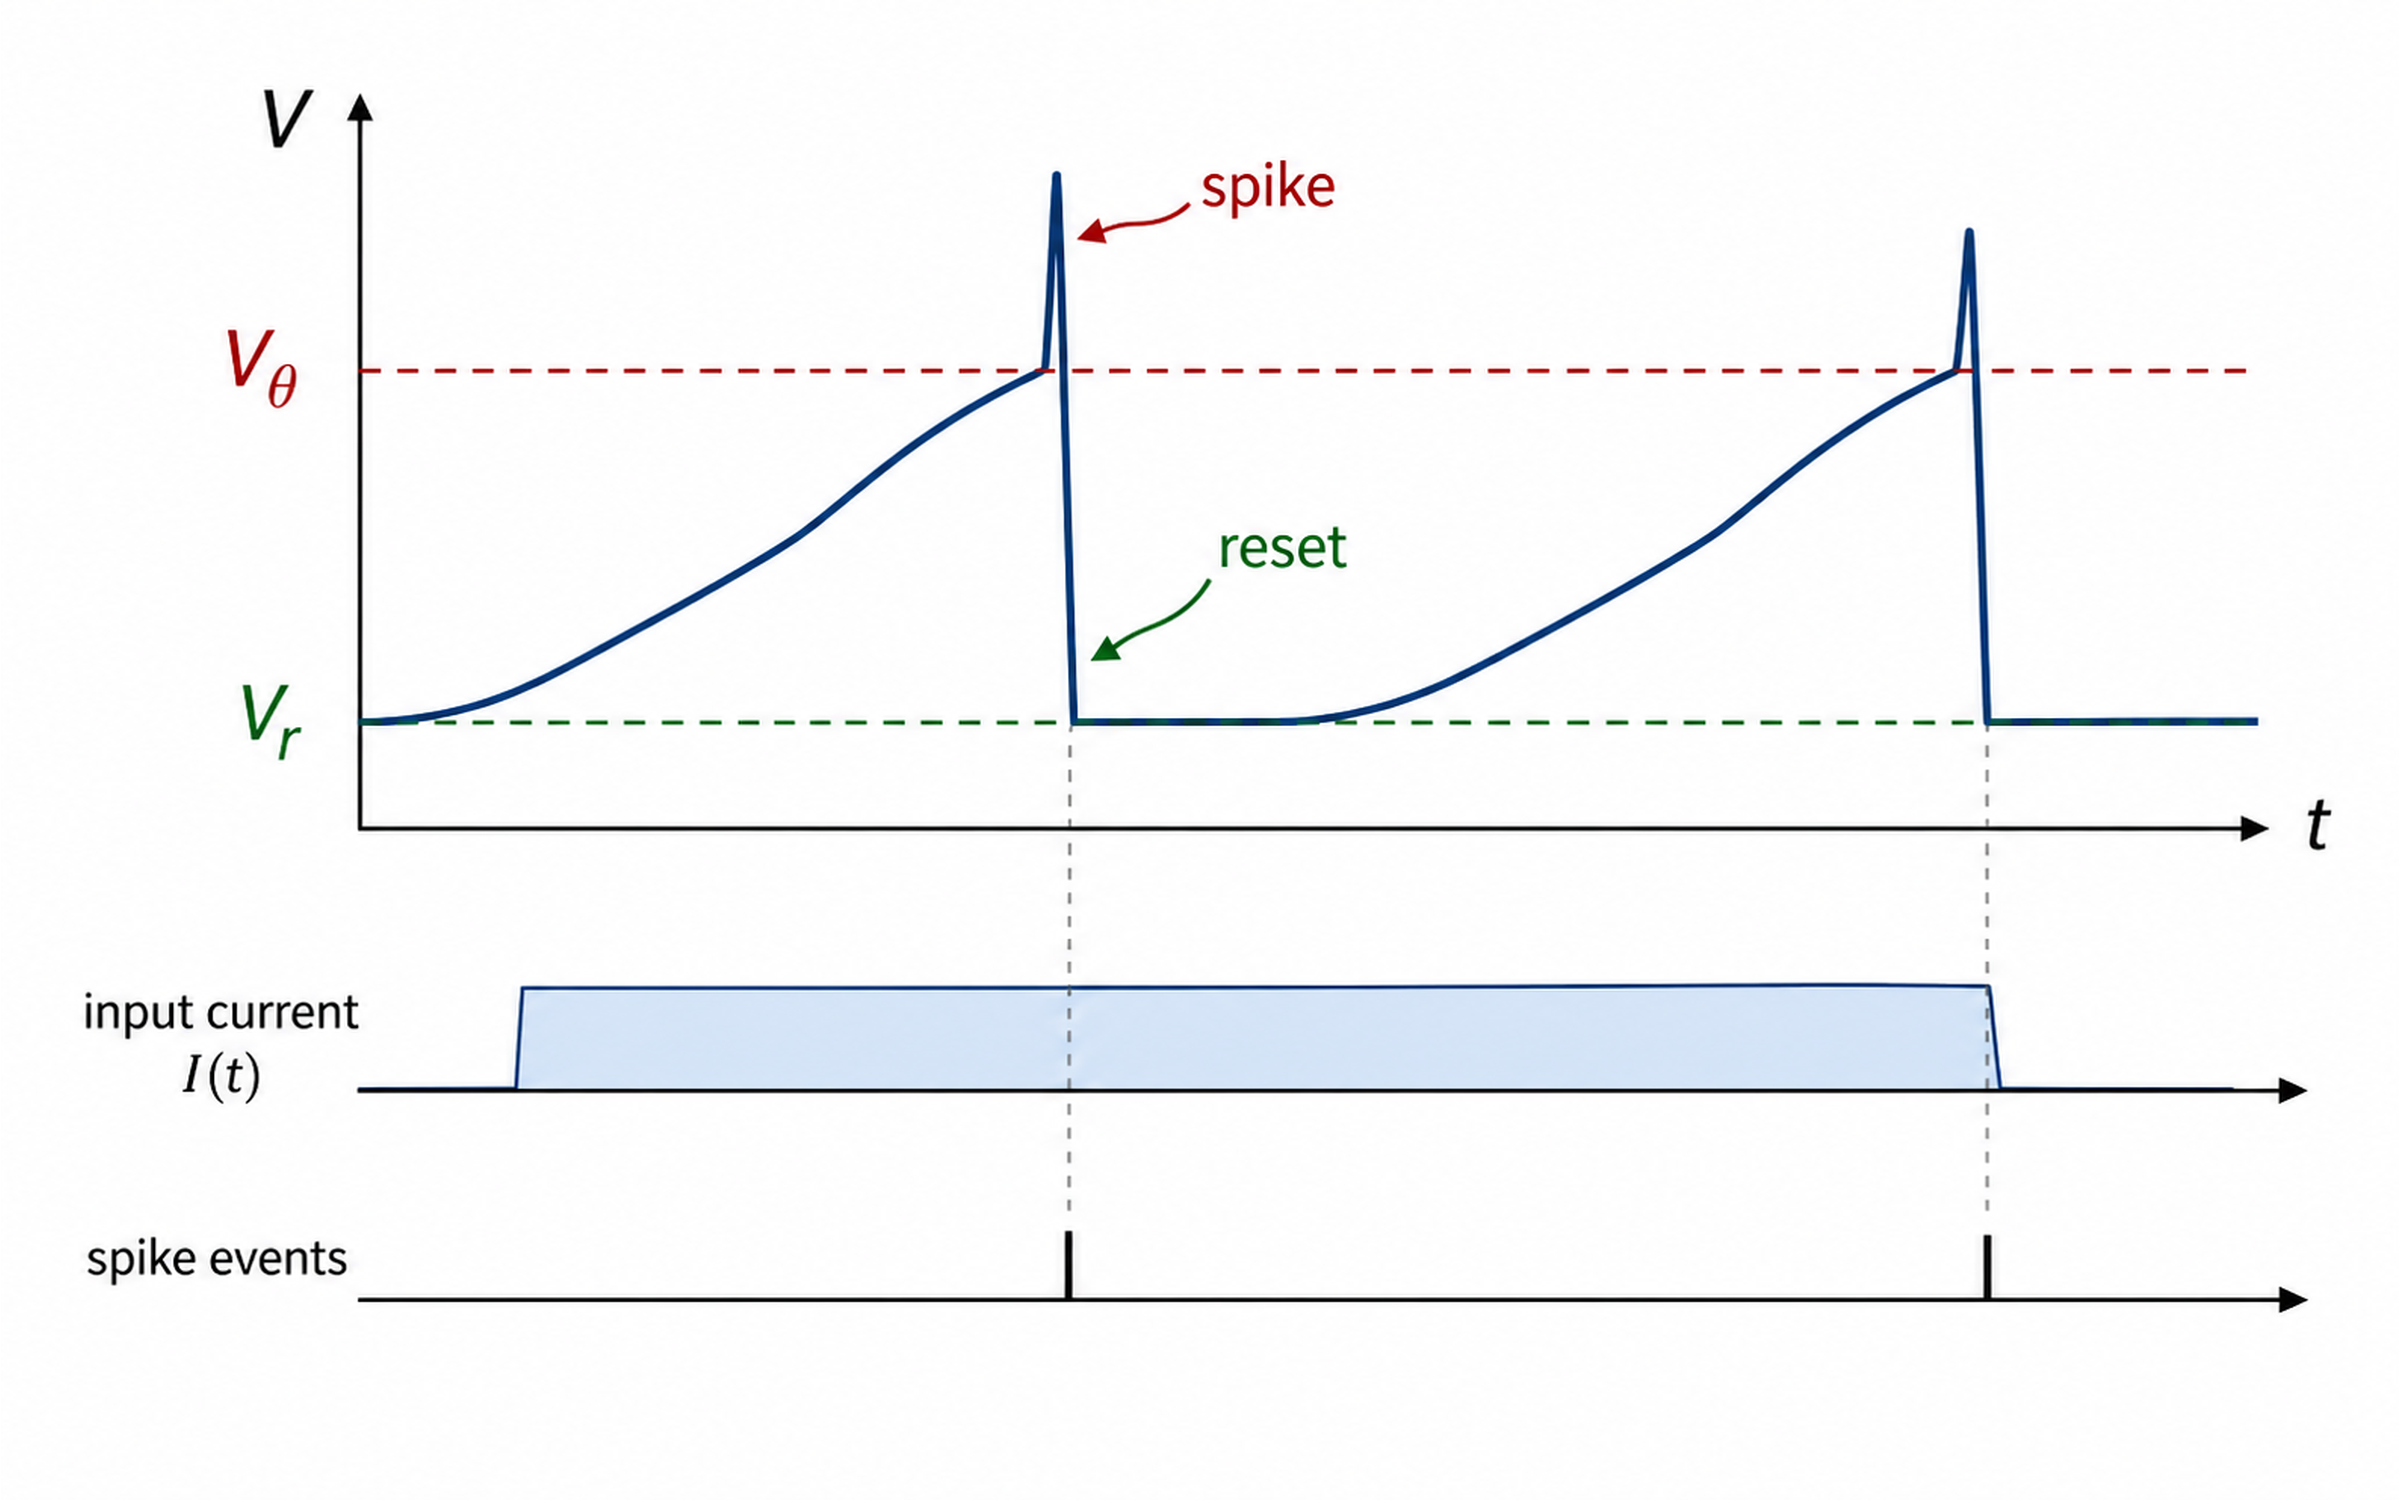
\includegraphics[width=0.88\textwidth]{figures/imagegen/ch03-lif-threshold-reset-img.png}
\caption{LIF voltage dynamics. Input current moves the membrane potential
toward threshold, a spike is emitted at $V_\theta$, and the reset $V_r$ creates
a short loss of memory. The figure emphasizes that spikes are events generated
by a continuous state variable, not values of a rate equation.}
\label{fig:ch03-lif-threshold-reset}
\end{figure}

If neuron $i$ spikes at times $\{t_{i,k}\}_{k\in\mathbb Z}$, its spike train is
the point process
%
\begin{equation}
  s_i(t) = \sum_k \delta(t-t_{i,k}).
  \label{eq:ch03-single-spike-train}
\end{equation}
%
This notation is compact but has a precise meaning: integrating $s_i(t)$ over a
time window counts spikes in that window. The voltage model determines the
event times; the spike train records them in the language needed for synaptic
input sums.

% ============================================================
\section{Synaptic Filtering and Stochastic LIF Neurons}
\label{sec:stochastic-lif}
% ============================================================

Presynaptic spikes do not become instantaneous postsynaptic voltage jumps in
the models used in the roadmap. They are first filtered by a synaptic kernel.
If the raw weighted input to neuron $i$ is $y_i(t)$, the current entering the
voltage equation can be written as
%
\begin{keyequation}[Filtered Synaptic Current]
\begin{equation}
  I_i(t)
  =
  \int_{-\infty}^{t} \epsilon(t-t')\,y_i(t')\,dt',
  \qquad
  \epsilon(t)=\frac{1}{\tau_s}e^{-t/\tau_s}H(t).
  \label{eq:ch03-filtered-current}
\end{equation}
\tcblower
$y_i(t)$: weighted sum of incoming spike trains; $\epsilon$: causal synaptic
filter; $\tau_s$: synaptic time constant; $H(t)$: Heaviside step function.
\end{keyequation}

\noindent The filter turns a delta spike into a postsynaptic current pulse. In
the roadmap this same operation is applied at the level of cluster inputs:
spike trains are summed, then smoothed by $\epsilon$. This is why activity
traces in clustered network simulations can be plotted as rates on tens of
milliseconds even though the microscopic variables are spikes.

Real cortical neurons also receive many unmodeled inputs. A standard way to
represent this unresolved drive is a stochastic LIF equation,
%
\begin{equation}
  \tau_m\,dV_i
  =
  \Bigl[-(V_i-E_L)+R_m I_i(t)\Bigr]\,dt
  + \sigma_V\sqrt{\tau_m}\,dW_i(t),
  \label{eq:ch03-stochastic-lif}
\end{equation}
%
where $W_i(t)$ is a Wiener process and $\sigma_V$ sets the voltage-noise scale.
The noise term should not be interpreted as a claim that all variability is
external. It is a coarse representation of many small fluctuating inputs, missing
synapses, and microscopic degrees of freedom that are not modeled explicitly.

Stochasticity changes the meaning of threshold. In the deterministic LIF model
a fixed input either produces a perfectly regular spike train or no spikes at
all. With noise, the same mean input produces a distribution of interspike
intervals. Threshold crossing becomes a first-passage problem: the next spike
time is the first time at which the random voltage trajectory reaches
$V_\theta$.

% ============================================================
\section{Escape Rates and Hazards}
\label{sec:escape-rates-hazards}
% ============================================================

For population theory it is often more convenient to replace the hard
threshold event by a conditional spike intensity. Given the neuron's current
state and spike history \(\mathcal H_t\), write
%
\begin{keyequation}[Escape-Rate Spike Probability]
\begin{equation}
  \Pr\{ dN_i(t)=1 \mid \mathcal H_t \}
  =
  \lambda_i(t\mid\mathcal H_t)\,dt + o(dt),
  \label{eq:ch03-escape-probability}
\end{equation}
\begin{equation}
  \lambda_i(t\mid\mathcal H_t)
  =
  h\!\left(
    V_i(t),\theta_i(t),z_i(t),t-\hat t_i
  \right).
  \label{eq:ch03-escape-rate-general}
\end{equation}
\tcblower
\(dN_i(t)\): infinitesimal spike count; \(\lambda_i\): hazard or escape rate;
\(h\): nonlinear escape function; \(z_i\): optional adaptation/filter
variables; \(\hat t_i\): most recent spike time; \(t-\hat t_i\): neuronal age.
\end{keyequation}
%
An escape-rate model does not discard the LIF/GIF state. It changes only the
last step: instead of a deterministic boundary crossing, the state controls a
probability per unit time. A common soft-threshold example is
%
\begin{equation}
  \lambda_i(t)
  =
  \lambda_0
  \exp\!\left(
    \frac{V_i(t)-\theta_i(t)}{\Delta V}
  \right)
  H(t-\hat t_i-\tau_{\mathrm{ref}}),
  \label{eq:ch03-soft-threshold-hazard}
\end{equation}
%
where \(\Delta V\) sets the sharpness of threshold and the Heaviside factor
enforces an absolute refractory time. Sending \(\Delta V\to 0\) recovers a hard
threshold in spirit, but the finite-\(\Delta V\) form is easier to average
over a population because it defines a smooth intensity.

This language connects directly to Chapter~\ref{ch:stochastic-processes-neural-dynamics}.
The conditional intensity of a point process is the single-neuron hazard. A
cluster activity equation will be obtained by averaging these hazards over all
neurons with the same cell type, cluster label, and age distribution.

% ============================================================
\section{Transfer Functions}
\label{sec:transfer-functions}
% ============================================================

A transfer function summarizes how a neuron responds to stationary input
statistics. Suppose the input is approximated by a mean drive $\mu$ and a
fluctuation scale $\sigma$. The stationary firing-rate transfer function is
defined by
%
\begin{keyequation}[Stationary Transfer Function]
\begin{equation}
  \phi(\mu,\sigma)
  =
  \lim_{T\to\infty}
  \frac{1}{T}\,
  \mathbb E\!\left[
    \int_0^T s_i(t)\,dt
    \,\middle|\,
    \mu,\sigma
  \right].
  \label{eq:ch03-transfer-function}
\end{equation}
\tcblower
$\phi(\mu,\sigma)$: expected spikes per unit time; $s_i(t)$: spike train;
$\mu$: mean input; $\sigma$: fluctuation amplitude; the expectation averages
over stochastic voltage paths or over repeated trials with the same input
statistics.
\end{keyequation}

\noindent This definition is deliberately statistical. It does not say that the
voltage is equal to $\phi$, and it does not say that one spike train is smooth.
It says that if a neuron is repeatedly driven with the same input statistics,
then its average spike count per unit time is approximately $\phi(\mu,\sigma)$.

\begin{figure}[t]
\centering
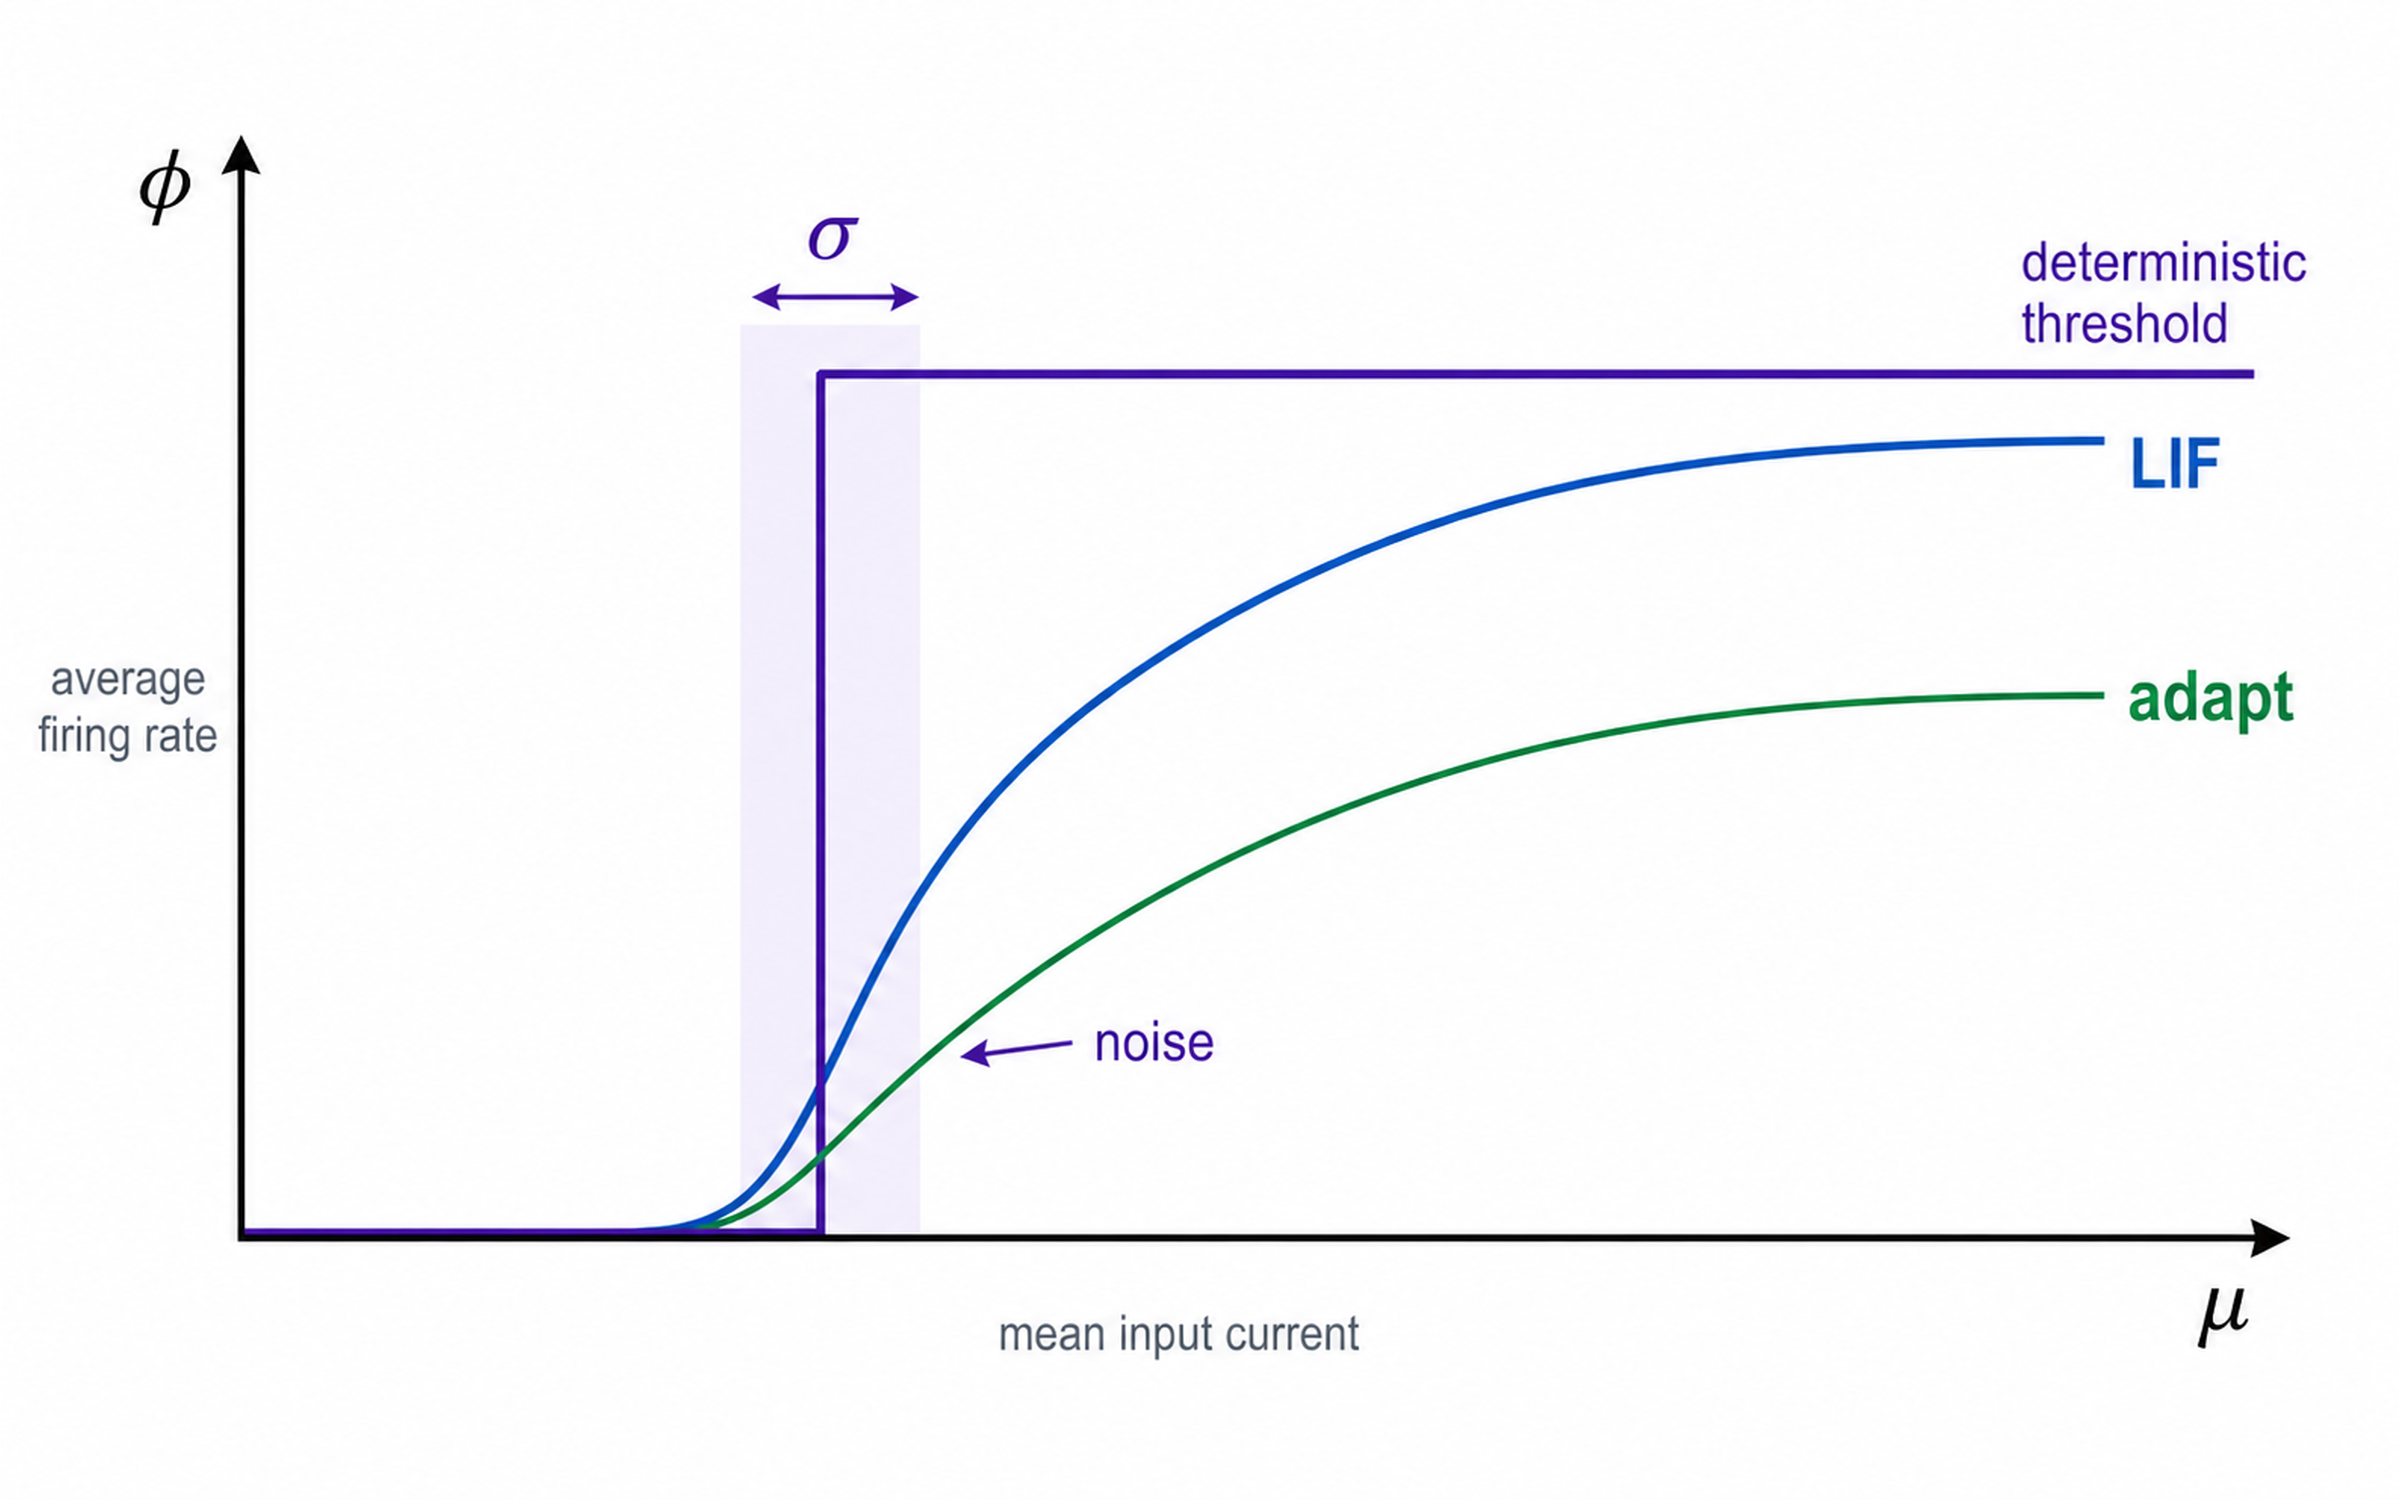
\includegraphics[width=0.88\textwidth]{figures/imagegen/ch03-transfer-function-img.png}
\caption{A transfer function maps input statistics to an expected firing rate.
Noise softens the deterministic threshold: inputs below the nominal threshold
can still elicit occasional spikes, and adaptation or GIF mechanisms can reduce
gain at high drive. The curve is a population or trial average, not a microscopic
state variable.}
\label{fig:ch03-transfer-function}
\end{figure}

Transfer functions are the bridge from spiking models to rate models. In a
network, the mean input to a neuron depends on the firing of other neurons.
Replacing a spiking population by a rate equation is therefore a self-consistent
approximation: assume an input statistic, compute the rate through $\phi$, feed
that rate back into the input, and solve for consistency. Later dynamic
mean-field theory will make the same idea time-dependent and stochastic.

% ============================================================
\section{Generalized Integrate-and-Fire Models}
\label{sec:gif}
% ============================================================

The LIF model is intentionally minimal. Generalized integrate-and-fire (GIF)
models keep the threshold/reset framework but add history dependence. A useful
schematic form is
%
\begin{align}
  \tau_m \frac{dV_i}{dt}
  &=
  -\bigl(V_i-E_L\bigr)
  - a_i(t)
  + R_m I_i(t),
  \label{eq:ch03-gif-voltage}
  \\
  \tau_a \frac{da_i}{dt}
  &=
  -a_i(t)
  + q_a \sum_k \delta(t-t_{i,k}),
  \label{eq:ch03-gif-adaptation}
  \\
  V_i(t^-)=\theta_i(t)
  &\Rightarrow
  \begin{cases}
    \text{emit a spike at }t,\\
    V_i(t^+)=V_r ,
  \end{cases}
  \qquad
  \theta_i(t)=\theta_0+\sum_{t_{i,k}<t}
  q_\theta e^{-(t-t_{i,k})/\tau_\theta}.
  \label{eq:ch03-gif-threshold}
\end{align}
%
The variable $a_i(t)$ is an adaptation current: after a spike it increases and
then decays, making immediate subsequent spikes less likely. Here $\tau_a$ is
the adaptation decay time and $q_a$ is the spike-triggered adaptation jump. The
dynamic threshold $\theta_i(t)$ is another form of refractoriness: $\theta_0$ is
the baseline threshold, $q_\theta$ is the threshold increase after each spike,
and $\tau_\theta$ is the relaxation time back toward baseline. The reset target
$V_r$ is the same kind of post-spike voltage used in the LIF rule, but in a GIF
model the neuron may also reset into a state with elevated adaptation current
and elevated threshold. Different GIF families use different filters, but the
principle is the same: the probability of a spike depends not only on the
current input, but also on recent spike history.

\begin{figure}[t]
\centering
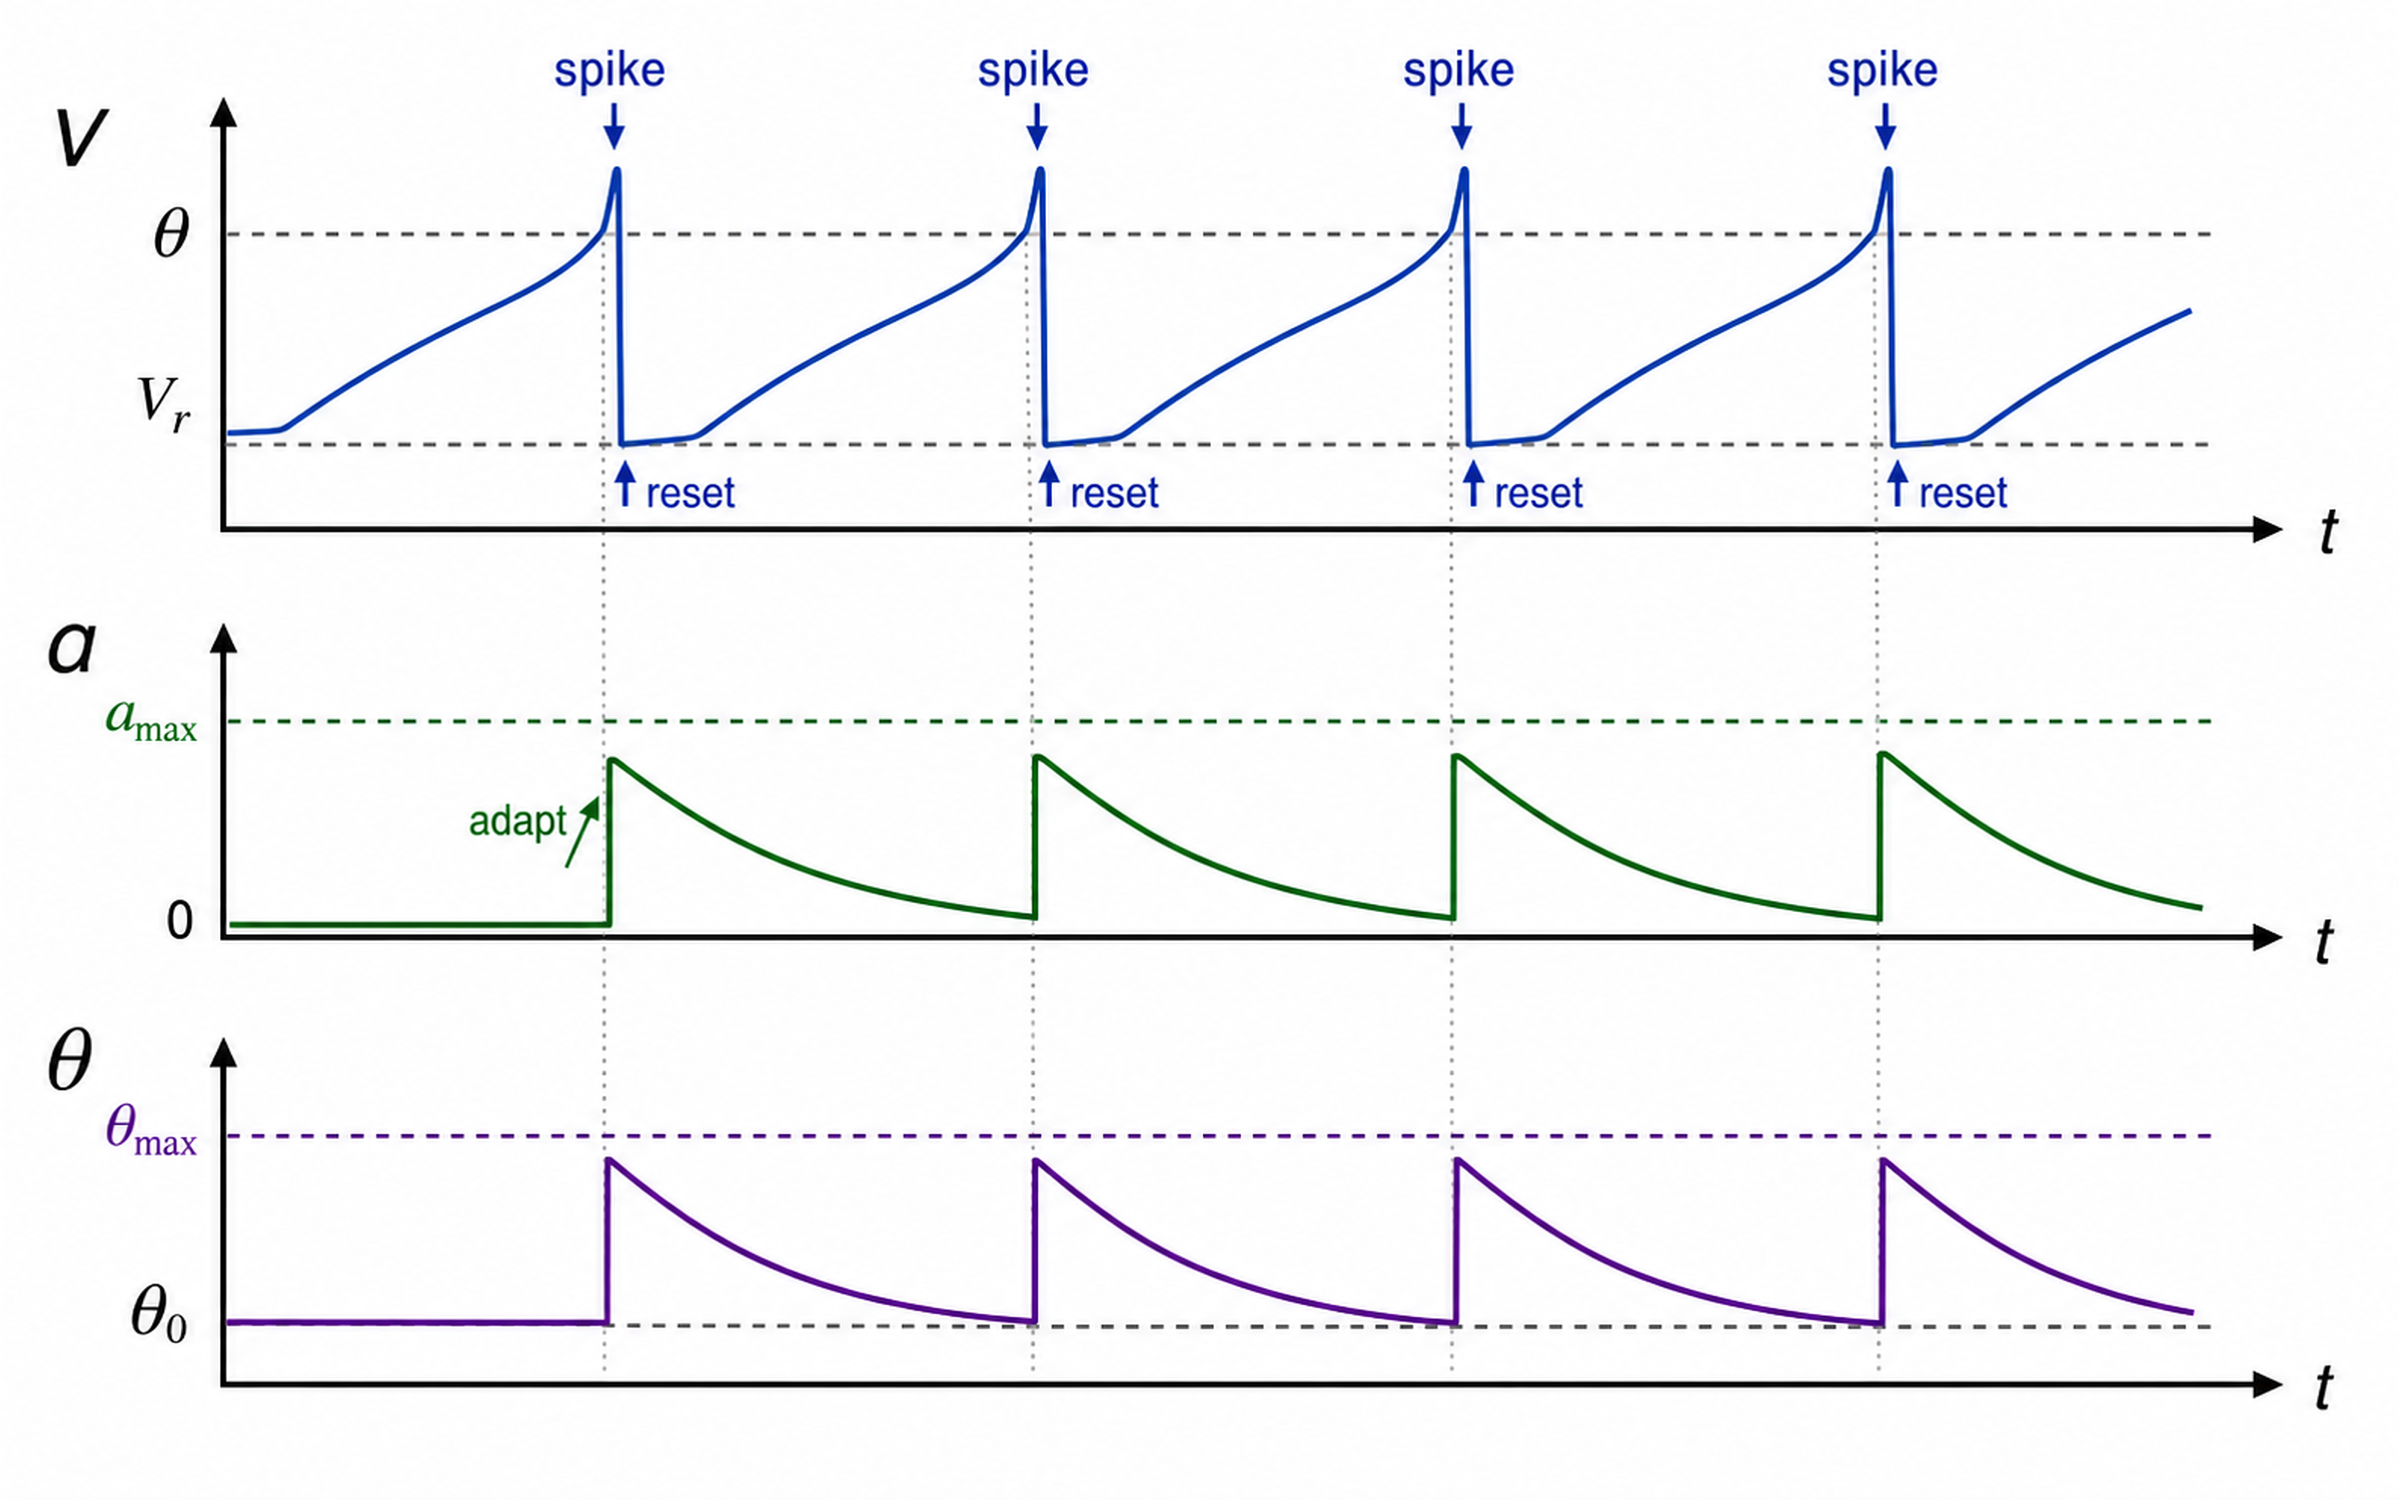
\includegraphics[width=0.90\textwidth]{figures/imagegen/ch03-gif-adaptation-img.png}
\caption{History dependence in a generalized integrate-and-fire neuron. Each spike can raise an adaptation current $a(t)$ and a dynamic threshold $\theta(t)$; both then relax back toward baseline. These extra state variables reduce near-term excitability and let GIF models match firing-rate statistics beyond the minimal LIF threshold-reset rule.}
\label{fig:ch03-gif-adaptation}
\end{figure}

GIF models are important for the clustered-network roadmap because they
provide a flexible microscopic spiking model without requiring detailed ion
channel dynamics. They can reproduce adaptation, refractoriness, and realistic
interspike-interval statistics while still being simple enough to embed in large
balanced networks.

% ============================================================
\section{Age Density and Renewal Activity Equations}
\label{sec:age-density-renewal}
% ============================================================

The finite-size population theory of Schwalger, Deger, and Gerstner
\citep{schwalgerDegerGerstner2017towards} starts from a simple observation:
after a spike, a neuron is not immediately exchangeable with one that has been
silent for a long time. The relevant coarse variable is therefore not only the
mean voltage or mean input. It is also the distribution of \emph{ages}, where
age \(\ell\) means time since the last spike.

Let \(q^\alpha(\ell,t)\,d\ell\) be the fraction of neurons of type \(\alpha\)
whose age lies in \([\ell,\ell+d\ell]\). If neurons of age \(\ell\) spike with
hazard \(\lambda^\alpha(\ell,t)\), then conservation of probability gives
%
\begin{keyequation}[Age-Density Population Equation]
\begin{align}
  \partial_t q^\alpha(\ell,t)
  + \partial_\ell q^\alpha(\ell,t)
  &=
  -\lambda^\alpha(\ell,t)q^\alpha(\ell,t),
  \qquad \ell>0,
  \label{eq:ch03-age-density-pde}
  \\
  q^\alpha(0,t)
  &=
  A^\alpha(t),
  \label{eq:ch03-age-density-boundary}
  \\
  A^\alpha(t)
  &=
  \int_0^\infty
  \lambda^\alpha(\ell,t)q^\alpha(\ell,t)\,d\ell,
  \qquad
  \int_0^\infty q^\alpha(\ell,t)\,d\ell=1.
  \label{eq:ch03-age-density-activity}
\end{align}
\tcblower
Neurons drift to larger age at unit speed. A fraction
\(\lambda^\alpha q^\alpha d\ell dt\) spikes, leaves its age bin, and re-enters
at age zero. The boundary value at \(\ell=0\) is the population activity.
\end{keyequation}

This equation is the cleanest bridge from single-neuron escape rates to
population activity. Refractoriness enters by making
\(\lambda^\alpha(\ell,t)=0\) for \(\ell<\tau_{\mathrm{ref}}\), or more
generally by lowering the hazard at small age. Input dependence enters because
\(\lambda^\alpha\) depends on filtered synaptic current, adaptation, and
possibly the recent population activity.

The same idea can be written in renewal form. If a neuron last spiked at
time \(t-\ell\), define the survival and interspike-interval density
%
\begin{align}
  S^\alpha(\ell\mid t-\ell)
  &=
  \exp\!\left[
    -\int_0^\ell
    \lambda^\alpha(u,t-\ell+u)\,du
  \right],
  \label{eq:ch03-survival}
  \\
  f^\alpha(\ell\mid t-\ell)
  &=
  \lambda^\alpha(\ell,t)S^\alpha(\ell\mid t-\ell).
  \label{eq:ch03-isi-density}
\end{align}
%
Then the activity at time \(t\) is the total contribution of neurons whose
previous spike occurred at \(t-\ell\) and whose next interval has length
\(\ell\):
%
\begin{equation}
  A^\alpha(t)
  =
  \int_0^\infty
  f^\alpha(\ell\mid t-\ell)
  A^\alpha(t-\ell)\,d\ell
  + A_{\mathrm{init}}^\alpha(t).
  \label{eq:ch03-renewal-activity}
\end{equation}
%
The initialization term carries neurons whose last spike happened before the
chosen start of the experiment. In stationary input it decays away, and the
mean firing rate reduces to the inverse mean interspike interval,
%
\begin{equation}
  \bar A^\alpha
  =
  \left[
    \int_0^\infty S^\alpha(\ell)\,d\ell
  \right]^{-1}.
  \label{eq:ch03-stationary-renewal-rate}
\end{equation}

For a GIF neuron, the exact hazard depends on more than the most recent spike:
adaptation and threshold kernels remember older spikes. The quasi-renewal
approximation keeps the most recent spike explicitly through the age \(\ell\)
and replaces older spikes by their expected contribution under the population
activity. For a spike-triggered threshold kernel \(\eta_\theta\), a useful
schematic form is
%
\begin{equation}
  \theta_{\mathrm{QR}}^\alpha(\ell,t)
  =
  \theta_0^\alpha
  + \eta_\theta^\alpha(\ell)
  + \int_\ell^\infty
  \eta_\theta^\alpha(s)A^\alpha(t-s)\,ds,
  \qquad
  \lambda^\alpha(\ell,t)
  \approx
  h_\alpha\!\left(U^\alpha(t)-\theta_{\mathrm{QR}}^\alpha(\ell,t)\right).
  \label{eq:ch03-quasi-renewal-threshold}
\end{equation}
%
The first kernel term is the refractory effect of the last spike; the integral
is the mean effect of earlier spikes. Different GIF implementations use more
careful kernels and correction factors, but the modeling move is the same:
replace a high-dimensional spike history by an age-resolved hazard that can be
advanced at the population level.

% ============================================================
\section{Finite-Size Population Activity Noise}
\label{sec:finite-size-population-noise}
% ============================================================

Equations~\eqref{eq:ch03-age-density-pde}--\eqref{eq:ch03-age-density-activity}
describe the infinite-population activity of one homogeneous population. A
finite population \(P\) of type \(\alpha\) contains \(N_P\) neurons, so the
empirical activity is
%
\begin{equation}
  A_{N_P}^\alpha(t)
  =
  \frac{1}{N_P}
  \sum_{i=1}^{N_P}s_i^\alpha(t).
  \label{eq:ch03-finite-empirical-activity}
\end{equation}
%
In this finite-size section, write \(A_\infty^\alpha(t)\) for the deterministic
infinite-population activity from the age-density equation, reserving
\(\bar A^\alpha\) for stationary renewal rates. Conditioned on the mesoscopic
state, the empirical spike count has sampling fluctuations. In a small bin of
width \(\Delta t\),
%
\begin{align}
  \mathbb E\!\left[
    A_{N_P,\Delta}^\alpha(t)
    \mid q^\alpha_t
  \right]
  &=
  A_\infty^\alpha(t),
  \label{eq:ch03-finite-bin-mean}
  \\
  \operatorname{Var}\!\left[
    A_{N_P,\Delta}^\alpha(t)
    \mid q^\alpha_t
  \right]
  &\approx
  \frac{A_\infty^\alpha(t)}{N_P\Delta t}.
  \label{eq:ch03-finite-bin-var}
\end{align}
%
The diffusion shorthand is therefore
%
\begin{keyequation}[Finite-Size Activity Approximation]
\begin{equation}
  A_{N_P}^\alpha(t)
  \approx
  A_\infty^\alpha(t)
  +
  \frac{1}{\sqrt{N_P}}
  \sqrt{A_\infty^\alpha(t)}\,\zeta^\alpha(t),
  \label{eq:ch03-activity-diffusion}
\end{equation}
\tcblower
\(\zeta^\alpha(t)\) is idealized white noise at the raw activity level. Renewal
statistics, refractoriness, common input, and recurrent coupling change its
temporal covariance; the robust scaling is the amplitude \(N_P^{-1/2}\).
\end{keyequation}

For a clustered E/I model, \(N_P=n_\alpha\). Thus
\[
  \xi_E=\frac{1}{\sqrt{n_E}},
  \qquad
  \xi_I=\frac{1}{\sqrt{n_I}},
\]
with a bare \(\xi\) usually meaning the excitatory cluster scale
\(\xi_E\). This is an annealed, dynamically resampled fluctuation. It is
different from quenched inter-cluster heterogeneity \(\kappa\), which is fixed
by the sampled connectivity or weights of the network realization.

Filtering converts the raw activity noise into the colored fluctuations seen
in rate traces. If \(R_{N_P}^\alpha=\epsilon*A_{N_P}^\alpha\) and
\(\epsilon(t)=\tau_s^{-1}e^{-t/\tau_s}H(t)\), then the independent stationary
Poisson baseline is
%
\begin{equation}
  C_{R_{N_P}^\alpha}(\tau)
  =
  \frac{\bar A^\alpha}{2\tau_s N_P}
  e^{-|\tau|/\tau_s}.
  \label{eq:ch03-filtered-finite-size-cov}
\end{equation}
%
This is not a universal covariance formula; it is the scale check. More
realistic renewal neurons have a different short-lag shape, and recurrent
networks can add shared fluctuations. For binned spike counts, let
\(\hat r_\Delta^\alpha\) denote the one-bin population rate estimator
\[
  \hat r_\Delta^\alpha
  =
  \frac{1}{N_P\Delta}
  \sum_{i=1}^{N_P}\int_t^{t+\Delta}s_i^\alpha(u)\,du.
\]
A compact way to see the effect of shared correlations is
%
\begin{equation}
  \operatorname{Var}\!\left[\hat r_\Delta^\alpha\right]
  =
  \frac{\bar A^\alpha}{N_P\Delta}
  +
  \frac{N_P-1}{N_P}
  c_\Delta^\alpha,
  \label{eq:ch03-shared-correlation-floor}
\end{equation}
%
where \(c_\Delta^\alpha\) is the average pairwise count covariance divided by
\(\Delta^2\). Independent neurons have \(c_\Delta^\alpha=0\). Positive shared
input or coherent cluster dynamics can leave a covariance floor that does not
look like independent sampling noise, so finite-size scaling must be measured,
not assumed.

% ============================================================
\section{Population Firing Rates}
\label{sec:population-rates}
% ============================================================

For a population $P$ containing $N_P$ neurons, the empirical population
activity is the average spike train
%
\begin{keyequation}[Population Activity and Filtered Rate]
\begin{equation}
  A_P(t)
  =
  \frac{1}{N_P}\sum_{i\in P} s_i(t),
  \qquad
  r_P(t)
  =
  \int_{-\infty}^{t}\epsilon(t-t')\,A_P(t')\,dt'.
  \label{eq:ch03-population-activity-rate}
\end{equation}
\tcblower
$A_P(t)$: spikes per neuron per unit time as a point process; $r_P(t)$:
synaptically filtered population rate; $N_P$: population size.
\end{keyequation}

\noindent For a paired E/I cluster the same definition becomes
%
\begin{equation}
  A_a^\alpha(t)
  =
  \frac{1}{n_\alpha}
  \sum_{i=1}^{n_\alpha}s_{a,i}^\alpha(t),
  \qquad
  R_a^\alpha(t)
  =
  (\epsilon*A_a^\alpha)(t),
  \qquad
  \alpha\in\{E,I\}.
  \label{eq:ch03-cluster-activity-rate}
\end{equation}
%
Here \(n_\alpha\) is the number of neurons of type \(\alpha\) in one cluster.
If a source formula writes \(N_E\) inside \(\xi=1/\sqrt{N_E}\), read that
\(N_E\) as the local count \(n_E\), not the total excitatory population
\(N_E^{\mathrm{tot}}\).

In code, the raw activity is usually represented by bins rather than literal
Dirac deltas. For bin width \(\Delta\),
%
\begin{equation}
  C_{a,m}^\alpha
  =
  \sum_{i=1}^{n_\alpha}
  \int_{m\Delta}^{(m+1)\Delta}
  s_{a,i}^\alpha(t)\,dt,
  \qquad
  \widehat A_{a,m}^\alpha
  =
  \frac{C_{a,m}^\alpha}{n_\alpha\Delta}.
  \label{eq:ch03-binned-cluster-activity}
\end{equation}
%
With an exponential filter and a piecewise-constant binned activity, the
filtered trace can be advanced by
%
\begin{equation}
  R_{a,m+1}^\alpha
  =
  e^{-\Delta/\tau_s}R_{a,m}^\alpha
  +
  \left(1-e^{-\Delta/\tau_s}\right)
  \widehat A_{a,m}^\alpha.
  \label{eq:ch03-filter-recursion}
\end{equation}
%
This is the practical microscopic-to-mesoscopic map used before computing
cluster lifetimes, autocorrelations, dimensionality, or perturbation
responses.

The same activity variables enter synaptic current equations. At the population
bookkeeping level,
%
\begin{equation}
  y_a^\alpha(t)
  =
  \sum_{\beta}
  n_\beta\widehat J^{\alpha\beta}A_a^\beta(t)
  +
  \sum_{b\ne a}\sum_{\beta}
  n_\beta\check J_{ab}^{\alpha\beta}A_b^\beta(t),
  \qquad
  I_a^\alpha=\epsilon*y_a^\alpha.
  \label{eq:ch03-population-input-map}
\end{equation}
%
Chapter~\ref{ch:ei-clustered-networks} will add the signs, balance scaling,
fixed in-degree variables, potentiation/depression factors, and quenched
heterogeneity. The important point here is that the same averaged spike trains
drive both the mesoscopic observables and the synaptic inputs.

\begin{center}
\renewcommand{\arraystretch}{1.35}
\begin{tabularx}{\textwidth}{@{}l X@{}}
  \toprule
  \textbf{Implementation step} & \textbf{Mathematical object} \\
  \midrule
  Record microscopic spikes &
  \(s_{a,i}^\alpha(t)=\sum_k\delta(t-t_{a,i,k}^\alpha)\) \\
  Bin by cluster and type &
  \(C_{a,m}^\alpha=\sum_i\int_{m\Delta}^{(m+1)\Delta}s_{a,i}^\alpha(t)\,dt\) \\
  Normalize by local population size &
  \(\widehat A_{a,m}^\alpha=C_{a,m}^\alpha/(n_\alpha\Delta)\) \\
  Filter to a continuous trace &
  \(R_a^\alpha=\epsilon*A_a^\alpha\), or the recursion in
  \eqref{eq:ch03-filter-recursion} \\
  Assign finite-size scale &
  \(\xi_\alpha=1/\sqrt{n_\alpha}\), with \(\xi=\xi_E\) when a single
  coordinate is used \\
  Separate quenched disorder &
  \(\kappa\) labels fixed network-to-network heterogeneity in
  \(\check J_{ab}^{\alpha\beta}\) or adjacency, not the spike sampling noise \\
  \bottomrule
\end{tabularx}
\end{center}

Averaging across neurons is what makes a smooth rate plausible. If neurons were
independent with comparable rates, the standard deviation of the population
average would scale as \(1/\sqrt{N_P}\). Correlations weaken this simple law,
but the scaling remains the baseline intuition: larger local populations have
smaller finite-size fluctuations. When later chapters speak of an active
cluster, they mean that a filtered population activity has moved to a high-rate
branch, not that every neuron in the cluster is firing regularly.

\begin{chaptersummary}
\begin{center}
\renewcommand{\arraystretch}{1.45}
\begin{tabularx}{\textwidth}{@{}l X X@{}}
  \toprule
  \textbf{Object} & \textbf{Equation} & \textbf{Interpretation} \\
  \midrule
  LIF voltage &
  $\tau_m \dot V=-(V-E_L)+R_m I$ &
  Continuous integration between spike events \\
  Spike train &
  $s_i(t)=\sum_k\delta(t-t_{i,k})$ &
  Event record generated by threshold crossings \\
  Synaptic filtering &
  $I=\epsilon*y$ &
  Spikes become postsynaptic current waveforms \\
  Escape rate &
  $\Pr\{dN(t)=1\mid\mathcal H_t\}=\lambda(t\mid\mathcal H_t)dt$ &
  Soft threshold or first-passage approximation for population theory \\
  Transfer function &
  $\phi(\mu,\sigma)=\lim_{T\to\infty}T^{-1}\mathbb E\int_0^T s(t)\,dt$ &
  Stationary input statistics mapped to expected rate \\
  Age-density activity &
  $A^\alpha(t)=\int_0^\infty\lambda^\alpha(\ell,t)q^\alpha(\ell,t)d\ell$ &
  Renewal bridge from refractory single neurons to population equations \\
  Finite-size activity &
  $A_N^\alpha\approx A_\infty^\alpha+N_P^{-1/2}\sqrt{A_\infty^\alpha}\zeta^\alpha$ &
  Leading empirical population noise, modified in shape by renewal statistics and correlations \\
  Population rate &
  $R_a^\alpha=\epsilon*A_a^\alpha$ &
  Cluster-rate observable obtained by averaging and smoothing microscopic spikes \\
  \bottomrule
\end{tabularx}
\end{center}
\end{chaptersummary}

\begin{conceptquestions}
  \item Why is a transfer function not the same kind of object as a membrane
  voltage? What averaging operation is hidden inside $\phi(\mu,\sigma)$?

  \item In the LIF model, where does the main nonlinearity enter: the
  subthreshold differential equation or the threshold/reset rule? Explain.

  \item How does stochastic drive change threshold crossing from a deterministic
  event into a first-passage problem?

  \item The population activity $A_P(t)$ is a sum of delta functions, while
  $r_P(t)$ is smooth. Which one is closer to the microscopic spike data, and
  which one is closer to the variables used in mean-field theory?

  \item Why should finite-size fluctuations decrease like $1/\sqrt{N_P}$ in an
  independent population? What kind of network effect could spoil the simplest
  version of that scaling?

  \item Starting from a GIF neuron with a spike-triggered threshold kernel,
  write the age-density equation and identify exactly where refractoriness
  changes the hazard.

  \item In a simulated paired E/I cluster with \(n_E=200\), \(n_I=50\), and
  \(\Delta=5\,\mathrm{ms}\), write the binned estimators
  \(\widehat A_{a,m}^E\) and \(\widehat A_{a,m}^I\). Which finite-size
  coordinate is the usual \(\xi\)?

  \item Suppose switching survives as \(n_E,n_I\) grow while the same
  inter-cluster weight realization is held fixed. Which term in this chapter's
  mesoscopic bridge becomes smaller, and which kind of mechanism remains
  plausible?
\end{conceptquestions}
